\documentclass{ieeeaccess}
\usepackage{cite}
\usepackage{amsmath,amssymb,amsfonts}
\usepackage{algorithmic}
\usepackage{graphicx}
\usepackage{textcomp}
\def\BibTeX{{\rm B\kern-.05em{\sc i\kern-.025em b}\kern-.08em
    T\kern-.1667em\lower.7ex\hbox{E}\kern-.125emX}}
\begin{document}
\history{Date of publication xxxx 00, 0000, date of current version xxxx 00, 0000.}
\doi{10.1109/ACCESS.2017.DOI}

\title{Joint Object Detection and Semantic Segmentation for Driving Safety of Personal Mobility Vehicle using Image-based Deep Learning Technique}

\author{\uppercase{Seungbo Shim}\authorrefmark{1, 2}, 
\uppercase{Gye-chun Cho}\authorrefmark{2}}
%\IEEEmembership{Member, IEEE}}
\address[1]{Future Infrastructure Research Center, Korea Institute of Civil Engineering and Build Technology (KICT), Goyang 10223, Korea }
\address[2]{Department of Civil and Environmental Engineering, Korea Advanced Institute of Science and Technology (KAIST), Daejeon 34141, Korea}
\tfootnote{This paragraph of the first footnote will contain support 
information, including sponsor and financial support acknowledgment. For 
example, ``This work was supported in part by the U.S. Department of 
Commerce under Grant BS123456.''}

\markboth
{Author \headeretal: Preparation of Papers for IEEE TRANSACTIONS and JOURNALS}
{Author \headeretal: Preparation of Papers for IEEE TRANSACTIONS and JOURNALS}

\corresp{Corresponding author: Gye-chun Cho (e-mail: gyechun@kaist.edu).}

\begin{abstract}
It will be updated.
\end{abstract}

\begin{keywords}
obstacle detection, road crack detection, joint learning, personal mobility, driving safety
\end{keywords}

\titlepgskip=-15pt

\maketitle

\section{Future mobility for the elderly and the disabled}
\label{sec:introduction}
\PARstart{A}{utonomous} personal mobility vehicles provide a convenient means of transportation for individuals. In particular, it will be a necessary vehicle of transportation for elderly people in the future as they enter an aging society. In general, elderly people have more difficulty driving the vehicle due to their ability to recognize obstacles compared to younger people \cite{b01}. Therefore, the dependence of autonomous vehicles will be high and the need for personal mobility vehicles will increase rather than autonomous vehicles because of the price \cite{b02}. This vehicle will become a means to encourage active social activities as well as an important technology that helps the disabled and the elderly who want to enjoy an independent life using safe and reliable means of transportation. Currently, Japan has already entered an unprecedented aging society. \cite{b03, b04}. As the number of young people decreases, the number of people engaged in production decreases significantly, and the transportation infrastructure necessary for people to live on is also constantly lacking. As a solution for these problems, the demand for personal mobility vehicles as a new means of transportation arises. In addition, electric wheelchairs and motor scooters has been on the rise recently amid social interest in improving the quality of life for the transportation for mobility handicapped. However, there is still a high possibility of accidents while driving, for those who have difficulty in making accurate judgments and rapid steering, such as the elderly and severely disabled. In order to reduce the possibility of such accidents and prevent them in advance, various sensors have been installed to require a means of transportation incorporating automated driving technology \cite{b05, b06}.

Various advanced sensors and related obstacle recognition technologies are required to reduce accidents in personal mobility \cite{b07}. Examples include technologies that enable proper recognition of obstacles such as vehicles, people, bicycles, motorcycles, etc. on the road. On the one hand, however, the individual transportation vehicle used by the elderly and the disabled are more affected by steering control depending on road surface conditions, since the wheel size is smaller than one of the car. Therefore, in situations where accidents occur depending on road conditions, small personal vehicle must be able to recognize road conditions in real time \cite{b08}. Recently, object recognition technology using artificial intelligence has been rapidly being applied to various fields, and technology to develop safe personal mobility is also expected to be used.


\section{related researches}
\label{sec:related researches}
\subsection{Obstacle detection during driving}
\label{subsec: obstacle deteciton}
A typical sensor used to detect dynamic obstacles that can be encountered while driving is Light Detection And Ranging (LiDAR). First, Teichamn et al.\cite{b09} proposed an algorithm to detect vehicles, people and bicycles using LiDAR. A 95\% accuracy was described in his research and tracks objects technology existing around the vehicle was addressed by installing sensors on top of the vehicle. Yi et al.\cite{b10} extracted profile features through a unsupervised algorithm, He used it to cluster target and recognize objects in the way based on Gaussian Mixture Model and Motion Compression. Azim et al.\cite{b11} proposed a method for simultaneously detecting and tracking the objects. He applied the Global Nearest Neighbor method to develop a general interface that can be connected with different kinds of sensors easily. Kaestner et al.\cite{b12} proposed a model that could recognized and tracked general target using 3D LiDAR. This showed the potential to recognize various objects.

Recently, sensor data obtained through LiDAR has been applied to deep learning frames to make significant advances in technology. These technologies are used primarily in the field of autonomous vehicles, which are largely categorized into two types. The first is the Projection-based method. For example, the LMNet\cite{b13} used front view projection techniques. Therefore, the two-dimensional feature from the three-dimensional input data was extracted using dilated convolution \cite{b14}, and it was used to recognize three-dimensional objects. However, this approach has an inevitable disadvantage of losing data in dimension reduction. To improve this, FVNet\cite{b15} used 3-channel front view projection method, moreover LaserNet\cite{b16} developed a technique for generating features with 5-channel.

The second is the Voxel-based method. The representative example is VoxelNet \cite{b17}. He proposed a voxel feature encoding method to make it possible to apply three-dimensional Convolutional neural network (CNN), and developed an deep learning neural network to perform feature extraction and boxing prediction in single stage. Chen et al.\cite{b19} combined 3D CNN and 2D CNN to reduce the loss of meaningful features. Also, Lehner et al.\cite{b20} constructed an algorithm based on a pillar-wise vertical feature, but furthermore, 2D Pseudo Bird Eye View map was used to increase recognition performance. Finally, Sualeh et al.\cite{b21} improved the completion of the recognition technology by developing an algorithm that tracks the movement path of the object through the fusion of the Interactive Multiple Model and the Unscented Kalman Filter\cite{b22} after 3D object recognition.

Another way to detect obstacles that may be encountered while driving is by using images. With the advent of deep learning, a plenty of studies has been introduced. These are largely divided into two-stage and one-stage structures. Object recognition technologies with a two-stage structure include Fast R-CNN \cite{b23}, Faster R-CNN \cite{b24}, and Mask R-CNN \cite{b25}. They created meaningful features for the target in the Backbone network, and then proposed candidate areas in the image where the target may exist. And finally, it used method of selecting the object region among these candidates. On the other hand, as object recognition technology with a one-stage structure, there are SSD \cite{b26}, YoloV3 \cite{b27}, RefineDet \cite{b28}, M2Det \cite{b29}, and so on. The focus was on increasing the computation speed by combining the steps of creating a candidate area expected to exist for these objects and determining the real area of the object. Those structure commonly have a step of extracting features from a backbone composed of a large number of layers to which CNN calculation is applied. This is because CNN operation assumes that the foreground and background features can be clearly distinguished. Each layer is connected by CNN operation and nonlinear activation function, and the unique feature is created as the depth increases. And based on the information obtained in this way, the type of algorithm varied depending on which method is applied to determine the location and type of the object in the image.

So far, various algorithms have been introduced according to the structure of deep neural networks in one input image. Next, we describe a technique for obtaining 3D information as well as obstacle detection by stereo images. Li et al.\cite{b30} used Faster R-CNN \cite{b24} to extract features from both left and right images and secures candidate groups that may have objects through the Region Proposal network. Next, a method of estimating a 3D box was proposed by adding a stereo regression block. Li et al. \cite{b31} proposed a lightweight 3D object recognition technique using 2D object recognition and an object tracking technique using spatial and temporal information. Chen et al. \cite{b32} applied an energy minimization technique to 3D object proposal generation using stereo vision. In addition, a method of using the generated information to estimate an object's pose and a two-dimensional bounding box was introduced.

The driving environment recognition technology examined so far is intended to be used in autonomous vehicles. This can be seen as a technology for preventing collision with a driving vehicle by recognizing an object with dynamic movement on the road. However, this is an appropriate technology for relatively big moving vehicles while driving, such as car, truck, bus. However, the situation is different for relatively small moving vehicles. When steering control is unstable during driving owing to the road surface condition, it is difficult to secure complete driving stability without road surface recognition technology.

\subsection{Surface damage detection on Road}
\label{subsec: surface damage}
Damage to road surfaces such as potholes seriously affects the driver's steering control. Although the impact may vary depending on the size and type of road surface damage, impact on the vehicle due to the pothole larger than tire's width may cause a traffic accident. The cause of road damage is due to natural factors caused by climate and temperature differences and aging due to continuous use. Therefore, it is practically impossible to prevent road surface damage in reality, then we have an interest on maintenance technology for quick repair. 

Regarding the road maintenance, researches on detecting road damage using images has been continuously done. Koch and Brilakis\cite{b33} used various image processing techniques to detect portholes, using histogram information and geometric information of the damaged area. In addition, they developed a recognition algorithm using morphological image processing techniques and asphalt material information. Buza et al.\cite{b34} used a spectral clustering method using histogram information extracted from gray image. Then he complete the algorithm to detect portholes using a sequential feature-based method of 9 steps. Jog et al.\cite{b35} proposed a method to reconstruct a 3D shape of pothole beyond recognizing road surface damage based on image information. The video taken continuously was divided into consecutive frames, and based on this, 3D reconstruction and modeling were performed to restore depth information of the real damaged area. Jo et al.\cite{b36} proposed algorithm to detect potholes using a sequential rule-based algorithm. He created a binary image, recognized the lane, and applied several filters to detect road damage with the assumption that pothole exists between the lanes. 

In the field of road surface detection using such images, studies through deep learning have begun to be introduced. Fan et al.\cite{b44} separated the input image into patches and applied several CNN and max-pooling operations. After passing through the Fully Connected Layer of step 3, binary images of 1×1 to 5×5 were obtained as output. Training was performed with a total of 96 images, and verified with 60 images. As a result, it was found to have an accuracy of more than 90\%. Jenkins et al.\cite{b37} used U-Net\cite{b38} based on the Auto-encoder method. He used data provided by the Crack Forest Dataset\cite{b45}, performed training with a total of 80 images, and verified with 20 images. then he showed F1-Score of 87.38\% result. Zou et al.\cite{b39} proposed an algorithm called DeepCrack. The feature of this algorithm was that the deep neural network was designed so that the weights were updated for each scale by using a skip-layer between the encoder and decoder steps. Bang et al \cite{b40} proposed a deep neural network algorithm in the form of an auto-encoder with images collected through a black box camera. For learning, 427 training images and 100 test images were secured by marking the crack area in the Full High Definition image. Using this, transfer learning-based training was performed, and as a result, the average accuracy was 77.68\%. Finally, Dhiman et al. \cite{b41} proposed an algorithm that detects potholes by combining deep learning technology and stereo vision.

However, until now, technology has been developed for the purpose of infrastructure maintenance in detecting road damage using images. As a result, the demand for real-time detection was insufficient, but it is obviously necessary to improve the computational speed for application to the autonomous driving field.

\subsection{Joint Deep Learning for driving safety}
\label{subsec: joint deep learning}
In this article we intend to propose an algorithm that not only recognizes dynamic obstacles encountered while driving on the road, but also recognizes the poor state of the road surface at a time. For this, we proposed a joint deep learning technique that can perform object detection and semantic segmentation at the same time. Researches developed so far in the field of autonomous driving \cite{b42, b43} has only detected the driving route by recognizing only the road area. This study assumed that the road surface always remains intact for driving. However, in reality, the road surface condition cannot be perfect, and a poor road surface can have a great influence on driving. In particular, since it can affect on personal mobility vehicles more sensitively, there is apparent need to detect both dynamic obstacles and road conditions simultaneously.











\begin{thebibliography}{00}

\bibitem{b01} A. Borowsky, D. Shinar, and T. Oron-Gilad, ``Age, skill, and hazard perception in driving,'' Accident Analysis and Prevention, vol. 42, no. 4, pp. 1240-1249, 2010.

\bibitem{b02}  M. Tinnilä and J. Kalli, ``Impact of future trends on personal mobility services,'' International Journal Automotive Technology and Management, vol. 15, no. 4, pp. 401–417, 2015.

\bibitem{b03} J. Nakane and M. Farevaag, ``Elder care in Japan,'' Perspectives (Gerontological Nursing Association (Canada)), vol. 28, no. 1, pp. 17-24, 2004.

\bibitem{b04} N. Muramatsu and H Akiyama, ``Japan: super-aging society preparing for the Future,'' The Gerontologist, vol. 51, no. 4, pp. 425–432, 2011.

\bibitem{b05} A. Argyros, P. Georgiadis, P. Trahanias and D. Tsakiris, ``Semi-autonomous navigation of a robotic wheelchair,'' Journal of Intelligent Robotic System, vol. 34, no. 3, pp. 315-329, 2002.

\bibitem{b06} Y. Kobayashi, Y. Kinpara, T. Shibusawa and Y. Kuno, ``Robotic wheelchair based on observations of people using integrated sensors,'' in Proc. 2009 IEEE/RSJ International Conference Intelligent Robots and Systems, St. Louis, MS, USA, pp. 2013-2018, Oct. 2009.

\bibitem{b07} C. Ilas, ``Electronic sensing technologies for autonomous ground vehicles: A review,'' in Proc. 8th International Symposium on Advanced Topics in Electrical Engineering (ATEE), Bucharest, Romania, pp. 1-6, May 2013.

\bibitem{b08} R. Madli, S. Hebbar, P. Pattar, and V. Golla, ``Automatic detection and notification of potholes and humps on roads to aid drivers,'' IEEE Sensors Journal, vol. 15, no. 8, pp. 4313-4318, 2015.

\bibitem{b09} A. Teichman, J. Levinson, and S. Thrun, ``Towards 3D object recognition via classification of arbitrary object tracks,'' in Proc. International Conference on Robotics and Automation (ICRA), pp. 4034–4041, May 2011.

\bibitem{b10} Y. Yi, Y. Guang, Z. Hao, F. Meng-yin, and W. Mei-ling, ``Moving object detection under dynamic background in 3D range data,'' in Proc. 2014 IEEE Intelligent Vehicles Symposium Proceedings, Ypsilanti, MI, USA, pp. 394-399, Jun. 2014.

\bibitem{b11} A. Azim and O. Aycard, ``Detection, classification and tracking of moving objects in a 3D environment,'' in Proc. 2012 IEEE Intelligent Vehicles Symposium, Alcala de Henares, Spain, pp. 802-807, Jun. 2012.

\bibitem{b12} R. Kaestner, J. Maye, Y. Pilat, and R. Siegwart, ``Generative object detection and tracking in 3D range data,'' in Proc. 2012 IEEE International Conference on Robotics and Automation, Saint Paul, MN, USA, pp. 3075-3081, May 2012.

\bibitem{b13} K. Minemura, H. Liau, A. Monrroy, and S. Kato, ``LMNet: real-time multiclass object detection on CPU using 3D LiDAR,'' in Proc. 3\textsuperscript{rd} Asia-Pacific Conference on Intelligent Robot Systems (ACIRS), Singapore, pp. 28-34, Jul. 2018.

\bibitem{b14} F. Yu and V. Koltun, ``Multi-scale context aggregation by dilated convolutions,'' 2015, arXiv:1511.07122. [Online]. Available: \underline{https://arxiv.org/abs/1511.07122}

\bibitem{b15} J. Zhou, X. Tan, Z. Shao, and L. Ma, ``FVNet: 3D front-view proposal generation for real-time object detection from point clouds,'' in Proc. 12\textsuperscript{th} International Congress on Image and Signal Processing, BioMedical Engineering and Informatics (CISP-BMEI), Suzhou, China, pp. 1-8, Oct. 2019.

\bibitem{b16} G. P. Meyer, A. Laddha, E. Kee, C. Vallespi-Gonzalez, and C. K. Wellington, ``LaserNet: an efficient probabilistic 3D object detector for autonomous driving,'' in Proc. IEEE/CVF Conference on Computer Vision and Pattern Recognition (CVPR), Long Beach, CA, USA, pp. 12669-12678, Jun. 2019.

\bibitem{b17} Y. Zhou and O. Tuzel, ``VoxelNet: End-to-End Learning for Point Cloud Based 3D Object Detection,'' in Proc. IEEE/CVF Conference on Computer Vision and Pattern Recognition, Salt Lake City, UT, USA, pp. 4490-4499, Jun. 2018.

% \bibitem{b18} Y Yan, Y Mao, and B Li, ``Second: sparsely embedded convolutional detection,'' Sensors, vol. 18, no. 10, e3337, 2018.

\bibitem{b19} Y. Chen, S. Liu, X. Shen, and J. Jia, ``Fast Point R-CNN,'' in Proc. IEEE/CVF International Conference on Computer Vision (ICCV), Seoul, Korea (South), pp. 9774-9783, Oct. 2019.

\bibitem{b20} J. Lehner, A. Mitterecker, T. Adler, M. Hofmarcher, B. Nessler, and S. Hochreiter, ``Patch refinement -- localized 3D object detection,'' 2019,  arXiv:1910.04093. [Online]. Available: \underline{https://arxiv.org/abs/1910.04093}

\bibitem{b21} M. Sualeh and G. W. Kim, ``Dynamic multi-LiDAR based multiple object detection and tracking,'' Sensors, vol. 19, no. 6, e1474, 2019.

\bibitem{b22} Q. Xu, X. Li, and C. Y. Chan, ``A cost-effective vehicle localization solution using an Interacting Multiple Model-Unscented Kalman Filters (IMM-UKF) algorithm and grey neural network,'' Sensors, vol. 17, no. 6, e1431, 2017.

\bibitem{b23} R. Girshick, ``Fast R-CNN,'' in Proc. IEEE International Conference on Computer Vision (ICCV), Santiago, Chile, pp. 1440-1448, Dec. 2015.

\bibitem{b24} S. Ren, K. He, R. Girshick, and J. Sun, ``Faster R-CNN: Towards Real-Time Object Detection with Region Proposal Networks,'' IEEE Transactions on Pattern Analysis and Machine Intelligence, vol. 39, no. 6, pp. 1137-1149, 2017.

\bibitem{b25} K. He, G. Gkioxari, P. Dollár, and R. Girshick, ``Mask R-CNN,'' in Proc. IEEE International Conference on Computer Vision (ICCV), Venice, Italy, pp. 2980-2988, Oct. 2017.

\bibitem{b26} W. Liu, D. Anguelov, D. Erhan, C. Szegedy, S. Reed, C.-. Fu, and A. C. Berg, ``SSD: Single shot multibox detector,'' in Proc. European Conference on Computer Vision (ECCV), Amsterdam, Netherlands, pp. 21-37, Oct. 2016.

\bibitem{b27} J. Redmon and A. Farhadi, ``YOLOv3: an incremental improvement,'' 2018, arXiv:1804.02767. [Online]. Available: \underline{https://arxiv.org/abs/1804.02767}

\bibitem{b28} S. Zhang, L. Wen, X. Bian, Z. Lei, and S. Z. Li, ``Single-shot refinement neural network for object detection,'' in Proc. IEEE/CVF Conference on Computer Vision and Pattern Recognition, Salt Lake City, UT, USA, pp. 4203-4212, Jun. 2018.

\bibitem{b29} Q. Zhao, T. Sheng, Y. Wang, Z. Tang, Y. Chen, L. Cai, and H. Ling, ``M2Det: a single-shot object detector based on multi-level feature pyramid network,'' in Proc. the AAAI Conference on Artificial Intelligence, Honolulu, HI, USA, pp. 9259-9266, Feb. 2019.

\bibitem{b30} P. Li, X. Chen, and S. Shen, ``Stereo R-CNN based 3D object detection for autonomous driving,'' in Proc. IEEE/CVF Conference on Computer Vision and Pattern Recognition (CVPR), Long Beach, CA, USA, pp. 7636-7644, Jun. 2019.

\bibitem{b31} P. Li, T. Qin, and S. Shen, ``Stereo vision-based semantic 3D object and ego-motion tracking for autonomous driving,'' in Proc. the European Conference on Computer Vision (ECCV),  Munich, Germany, pp. 646-661, Sep. 2018. 

\bibitem{b32} X. Chen, K. Kundu, Y. Zhu, H. Ma, S. Fidler, and R. Urtasun, ``3D object proposals using stereo imagery for accurate object class detection," IEEE Transactions on Pattern Analysis and Machine Intelligence, vol. 40, no. 5, pp. 1259-1272, 2018.

\bibitem{b33} C. Koch and I. Brilakis, ``Pothole detection in asphalt pavement images,'' Advanced Engineering Informatics, vol. 25, no. 1, pp.507-515, 2011.

\bibitem{b34} E. Buza, S. Omanovic, and A. Huseinovic, ``A pothole detection with image processing and spectral clustering,'' in Proc. the 2\textsuperscript{nd} International Conference on Information Technology and Computer Networks, Antalya, Turkeys, pp. 48-53, Oct. 2013.

\bibitem{b35} G. M. Jog, C. Koch, M. Golparvar-Fard, and I. Brilakis, ``Pothole properties measurement through visual 2D recognition and 3D reconstruction,'' Computing in Civil Engineering, pp. 553-560, 2012.

\bibitem{b36} Y. Jo, S. K. Ryu, and Y. R. Kim, ``Pothole detection based on the features of intensity and motion,'' Journal of the Transportation Research Board, no. 2595, pp. 18-28, 2016.

\bibitem{b37} M. D. Jenkins, T. A. Carr,  M. I. Iglesias, T. Buggy, G. and Morison, ``A deep convolutional neural network for semantic pixel-wise segmentation of road and pavement surface cracks,'' in Proc. 26th European Signal Processing Conference (EUSIPCO), Rome, Italy, pp. 2120-2124, Sep. 2018.

\bibitem{b38} O. Ronneberger, P. Fischer, and T. Brox, ``U-net: Convolutional networks for biomedical image segmentation,'' in Proc. International Conference on Medical Image Computing and Computer-Assisted Intervention (MICCAI), Munich, Germany, pp. 234-241, Oct. 2015.

\bibitem{b39} Q. Zou, Z. Zhang, Q. Li, X. Qi, Q. Wang, and S. Wang, ``DeepCrack: Learning hierarchical convolutional features for crack detection,'' IEEE Transactions on Image Processing, vol. 28, no. 3, pp. 1498-1512, 2019.

\bibitem{b40} S. Bang, S. Park, H. Kim, and H. Kim, ``Encoder–decoder network for pixel‐level road crack detection in black‐box image,''  Computer Aided Civil and Infrastructure Engineering, vol. 34, no. 8, pp. 713-727, 2019.

\bibitem{b41} A. Dhiman and R. Klette, ``Pothole Detection Using Computer Vision and Learning,'' IEEE Transactions on Intelligent Transportation Systems, vol. 21, no. 8, pp. 3536-3550, 2020.

\bibitem{b42} D. Feng, C. Haase-Schütz, L. Rosenbaum, H. Hertlein, C. Gläser, F. Timm, W. Wiesbeck, and K. Dietmayer, "Deep Multi-Modal Object Detection and Semantic Segmentation for Autonomous Driving: Datasets, Methods, and Challenges," IEEE Transactions on Intelligent Transportation Systems, 2020.

\bibitem{b43} L. Chen, Z. Yang, J. Ma, and Z. Luo, ``Driving Scene Perception Network: Real-Time Joint Detection, Depth Estimation and Semantic Segmentation,'' in Proc. IEEE Winter Conference on Applications of Computer Vision (WACV), Lake Tahoe, NV, USA, pp. 1283-1291, Mar. 2018.

\bibitem{b44} Z. Fan, Y. Wu, J. Lu, and W. Li, ``Automatic pavement crack detection based on structured prediction with the convolutional neural network,'' 2018, arXiv:1802.02208. [Online]. Available: \underline{https://arxiv.org/abs/1802.02208}

\bibitem{b45} Y. Shi, L. Cui, Z. Qi, F. Meng, and Chen Z., ``Automatic road crack detection using random structured forests,'' IEEE Transactions on Intelligent Transportation Systems, vol. 17, no. 12, pp. 3434–3445, 2016.


\end{thebibliography}

\begin{IEEEbiography}[{
\includegraphics[width=1in,height=1.25in,clip,keepaspectratio]{fig/Shim_pic.jpg}}]{Seungbo Shim} was born in Donghae, Republic of Korea in 1982. He received the B.S. degree in electrical engineering from Pusan National University, Pusan, South Korea, in 2009 and the M.S. degree in electronic and electrical engineering from Pohang University of Science and Technology (POSTECH),Pohang, South Korea, in 2011.
From 2010 to 2017, he was a research engineer with Samsung Heavy Industries. Since 2017, he has been a research specialist with Korea Institute of Civil Engineering and Building Technology. Also, he is currently pursuing the Ph. D. degree in Korea Advanced Institute of Science and Technology from 2020. His current interests include machine vision, deep learning, automatic measurement system, sensor network, and infrastructure maintenance.
\end{IEEEbiography}

\begin{IEEEbiography}[{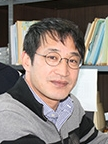
\includegraphics[width=1in,height=1.25in,clip,keepaspectratio]{fig/Cho.jpg}}]{Gye-Chun Cho} was born in South Korea in 1970. He received the B.S. degree in civil engineering in 1994 and the M.S. degree in geotechnical engineering in 1996 from Korea University, Seoul, South Korea. Also, he received the Ph. D degree in geotechnical engineering from Georgia Institute of Technology, GA, USA, in 2001. He was a assistant professor in Pennsylvania State University, PA, USA, from 2001 to 2002, and an assistant professor in Korea Advanced Institute of Science and Technology (KAIST), Daejeon, South Korea, from 2002 to 2005, and an associate professor in KAIST from 2005 to 2012, and a visiting professor in Georgia Institute of Technology from 2009 to 2010. Since 2012, he has been a professor with the Department of Civil and Environmental Engineering, KAIST. His current research interests include infrastructure maintenance, tunnel excavation, biopolymers, and soil behavior analysis. 
\end{IEEEbiography}

\EOD

\end{document}
